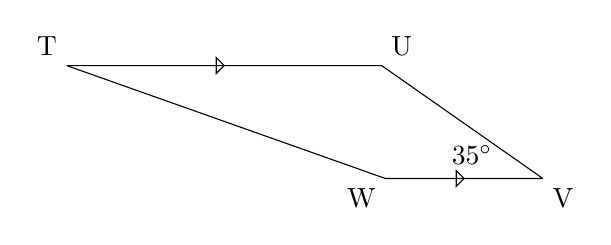
\begin{tikzpicture}
\draw(0,3)node[anchor=south east]{T}--(4,3)node[anchor=south
west]{U}--++(325:2.5)node[anchor=north west]{V}++(-0.9,0.3)node{$35^{\circ}$}++(0.9,-0.3)--++(-2,0)node[anchor=north east]{W}--(0,3);
\draw(2,3)--+(-.1,.1)--+(-.1,-.1)--cycle;
\draw(4,3)++(325:2.5)++(-1,0)--+(-.1,.1)--+(-.1,-.1)--+(0,0);
\end{tikzpicture}
\begin{center}
Note: diagram is \textbf{NOT} to scale.
\end{center}
In quadrilateral TUVW,  $\overline{TU} \| \overline{VW}$. If $ m\angle V$ measures 35 degrees, what is $m\angle T - m\angle U + m\angle V + m\angle W$?



\ifsat
	\begin{enumerate}[label=\Alph*)]
		\item  $35^{\circ}$
		\item  $70^{\circ}$%
		\item  $145^{\circ}$
		\item  $325^{\circ}$
	\end{enumerate}
\else
\fi

\ifacteven
	\begin{enumerate}[label=\textbf{\Alph*.},itemsep=\fill,align=left]
		\setcounter{enumii}{5}
		\item  $35^{\circ}$
		\item  $70^{\circ}$%
		\item  $145^{\circ}$
		\addtocounter{enumii}{1}
		\item  $180^{\circ}$
		\item  $325^{\circ}$
	\end{enumerate}
\else
\fi

\ifactodd
	\begin{enumerate}[label=\textbf{\Alph*.},itemsep=\fill,align=left]
		\item  $35^{\circ}$
		\item  $70^{\circ}$%
		\item  $145^{\circ}$
		\item  $180^{\circ}$
		\item  $325^{\circ}$
	\end{enumerate}
\else
\fi

\ifgridin
  $70^{\circ}$%
		
\else
\fi

